\documentclass[twocolumn]{aastex63}

% typography
\usepackage[T1]{fontenc}

\usepackage{amsmath}

\setlength{\parindent}{1.\baselineskip}
\newcommand{\acronym}[1]{{\small{#1}}}
\newcommand{\package}[1]{\textsl{#1}}
\newcommand{\gaia}{\textsl{Gaia}}
% \newcommand{\hst}{\textsl{HST}}
% \newcommand{\pans}{\textsl{Pan-STARRS}}

% \newcommand{\deg}{\ensuremath{\textrm{deg}}}
\newcommand{\kpc}{\ensuremath{\textrm{kpc}}}
\newcommand{\ul}{\ensuremath{\textrm{kpc}^2\,\textrm{Myr}^{-1}}}
\newcommand{\ue}{\ensuremath{\textrm{kpc}^2\,\textrm{Myr}^{-2}}}
\newcommand{\kms}{\ensuremath{\textrm{km}\,\textrm{s}^{-1}}}
\newcommand{\masyr}{\ensuremath{\textrm{mas}\,\textrm{yr}^{-1}}}
\newcommand{\feh}{\ensuremath{\textrm{[Fe/H]}}}
\newcommand{\afe}{\ensuremath{\textrm{[$\alpha$/Fe]}}}

\newcommand{\changes}[1]{{\textbf{#1}}}
\hyphenation{kruijs-sen}

% aastex parameters
% \received{not yet; THIS IS A DRAFT}
%\revised{not yet}
%\accepted{not yet}
% % Adds "Submitted to " the arguement.
% \submitjournal{ApJ}
\shorttitle{}
\shortauthors{bonaca et al.}

%@arxiver{}

\begin{document}\sloppy\sloppypar\raggedbottom\frenchspacing % trust me

\title{Phase-space Clustering Identifies the Origin of Galactic Stellar Streams}

\correspondingauthor{Ana~Bonaca}
\email{ana.bonaca@cfa.harvard.edu}

\author[0000-0002-7846-9787]{Ana~Bonaca}
\affil{Center for Astrophysics | Harvard \& Smithsonian, 60 Garden Street, Cambridge, MA 02138, USA}

\author{coauthors}

% \author[0000-0002-8804-0212]{J.~M.~Diederik~Kruijssen}
% \affiliation{Astronomisches Rechen-Institut, Zentrum f\" ur Astronomie der Universit\" at Heidelberg, M\" onchhofstra\ss e 12-14, D-69120 Heidelberg, Germany}
% \affil{Center for Astrophysics | Harvard \& Smithsonian, 60 Garden Street, Cambridge, MA 02138, USA}


\begin{abstract}\noindent % trust me
Many stellar streams, remnants of globular clusters and dwarf galaxies disrupted in the Milky Way, lack a discernible progenitor.
With the vast improvement in the precision of proper motions provided by Gaia EDR3, we show that the orbits of 23 Galactic stellar streams are extremely clustered in the orbital phase space.
Based on their energies and angular momenta, all streams in our sample can plausibly be associated with a dwarf galaxy host that brought them into the Milky Way.
For several streams we additionally identify globular cluster progenitors.
Surprisingly, these stream progenitors are displaced from their tidal debris by XX degrees.
Finally, we identify stellar streams that appear spatially distinct, but whose similar orbits indicate they likely originate from the same progenitor.
If confirmed as physical discontinuities, they will provide strong constraints on the mass-loss rate from the progenitor, and possibly regions of chaotic dispersal in the Galaxy.
The universal ex-situ origin of stellar streams we analyzed makes them exquisite tracers of galaxy mergers and dynamical friction.
Their phase-space clustering can be leveraged to construct a precise global map of dark matter in the Milky Way, while their structure may hold clues to the small-scale structure of dark matter in their original host galaxies.
% : Fimbulthul with Thamnos; GD-1, Gj\" oll, Leiptr, Phlegethon, Wambelong, and Ylgr with Sequoia / Arjuna / I'itoi; Ophiuchus with Gaia-Enceladus; Aliqa Uma, ATLAS, Elqui, Slidr, Sylgr, and Turranburra with Sagittarius; Fjorm, and Turbio with Helmi Streams; Indus, Jhelum, Phoenix, Ravi, and Sv\" ol with Wukong; and Triangulum and Willka Yaku with Cetus.
% (Omega Cen---Fimbulthul, NGC~3201---Gj\" oll, NGC~4590---Fjorm, NGC~5024---Sylgr and Ravi, NGC~5272---Sv\" ol, NGC~5824---Triangulum).
% - connected to gcs
% Frequent associations of streams to bound clusters may indicate a rapid dispersal following the full dissolution of the progenitor cluster, while 
% have orbits similar to those of surviving globular clusters, despite being spatially offset from them.
% their spatial offset is potentially a signature of episodic mass loss.
\end{abstract}

\keywords{%
stars:~kinematics~and~dynamics
  ---
Galaxy:~halo
  ---
Galaxy:~kinematics~and~dynamics
}

\section{Introduction}
\label{sec:intro}

- streams observed messed up

- happened in the mw or inherited from the host?
- can't tell since we don't know the origin

- for stars and gc: ex-situ identified from their orbital properties

- been hard for streams bc most stars faint, couldn't do good orbits
- but then edr3 happened
- present here elz for streams

% Hypotheses:
% \begin{itemize}
% \item{We can associate streams with the Milky Way progenitor galaxies.}
% \item{Streams are clumped at the center of the progenitor with which they were accreted. Streams were dissolved because they experienced stronger tidal field than clusters stripped out at higher energies (which is why they remain bound until today). This explains why streams are clumpy in the phase-space, while globular clusters are not.}
% \item{Strength of Milky Way's tidal field at this location equals the gravitational pull of the progenitor, which is why everything fell apart here. Therefore, we can read off the mass of the progenitor from this location, and compare that to the neural net estimates.}
% \item{The span in angular momentum (and energy?) of clusters and streams is set by dynamical friction the progenitor experienced, which provides another way to estimate the mass of the progenitor galaxy.}
% \item{The energy of the progenitor's center (stream clump) maps to the accretion redshift.}
% \item{A massive globular cluster close to a stream clump was likely this progenitor's nuclear star cluster.}
% \item{Given our better understanding of the trail a galaxy leaves in the phase space, we can also update globular cluster and stream associations previously reported. Based on that, it seems like we have another retrograde progenitor in addition to Sequoia!}
% \item{Based on their proximity in the phase space, at least some streams considered so far as individual objects, may in fact be different parts of the same structure.}
% \end{itemize}
% 
% Puzzles / spin-offs:
% \begin{itemize}
% \item{Why are both prograde and retrograde progenitors leaving trails like \textbackslash \textbackslash\ instead of \textbackslash\ /?}
% \item{It seems that there are some gaps in the phase space, both in the distribution of streams and clusters, and H3 stars. Are these just well-separated, distinct progenitors?}
% \item{Taking uncertainties into account, are the stream clumps actually distinct? (How strongly) Can we rule out a uniform distribution?}
% \item{Can we use metallicity of streams and field stars in this analysis? Do we expect it to follow the globular cluster trail?}
% \item{How are EMOSAICS clusters distributed in the phase space?}
% \end{itemize}

\section{Stream Orbit Fits}
In this work we use stream orbits derived by \citet{bk2021}, and in this section provide a high-level overview of their fitting procedure.
Positions and velocities of stream stars trace the orbit of their progenitor \citep[e.g.,][]{kuepper2010}.
Thanks to data released by the \gaia\ mission, 3D positions and two proper motion components are known for a sample of 23 streams without a discernible progenitor \citep{ibata2019, shipp2019, riley2020}.
Radial velocities have been measured for five of these streams for full 6D phase-space information \citep{caldwell2020, li2020, bonaca2020b}.

Assuming a static, axisymmetric model of the Milky Way \citep[default \texttt{MilkyWayPotential}]{gala}, \citet{bk2021} used these stream data to constrain their orbits.
They sampled the stream orbital parameters using a Monte Carlo Markov Chain ensemble sampler and provide direct samples from the posterior to account for correlations between parameters.
In this work we characterize the orbit by its total energy, $E_{\rm tot}$, and the $z$ component of the angular momentum, $L_z$ (perpendicular to the Galactic disk)---both conserved quantities in the adopted gravitational potential.
We use a right-handed coordinate system, such that $L_z<0$ denotes prograde orbits.

\begin{figure*}
\begin{center}
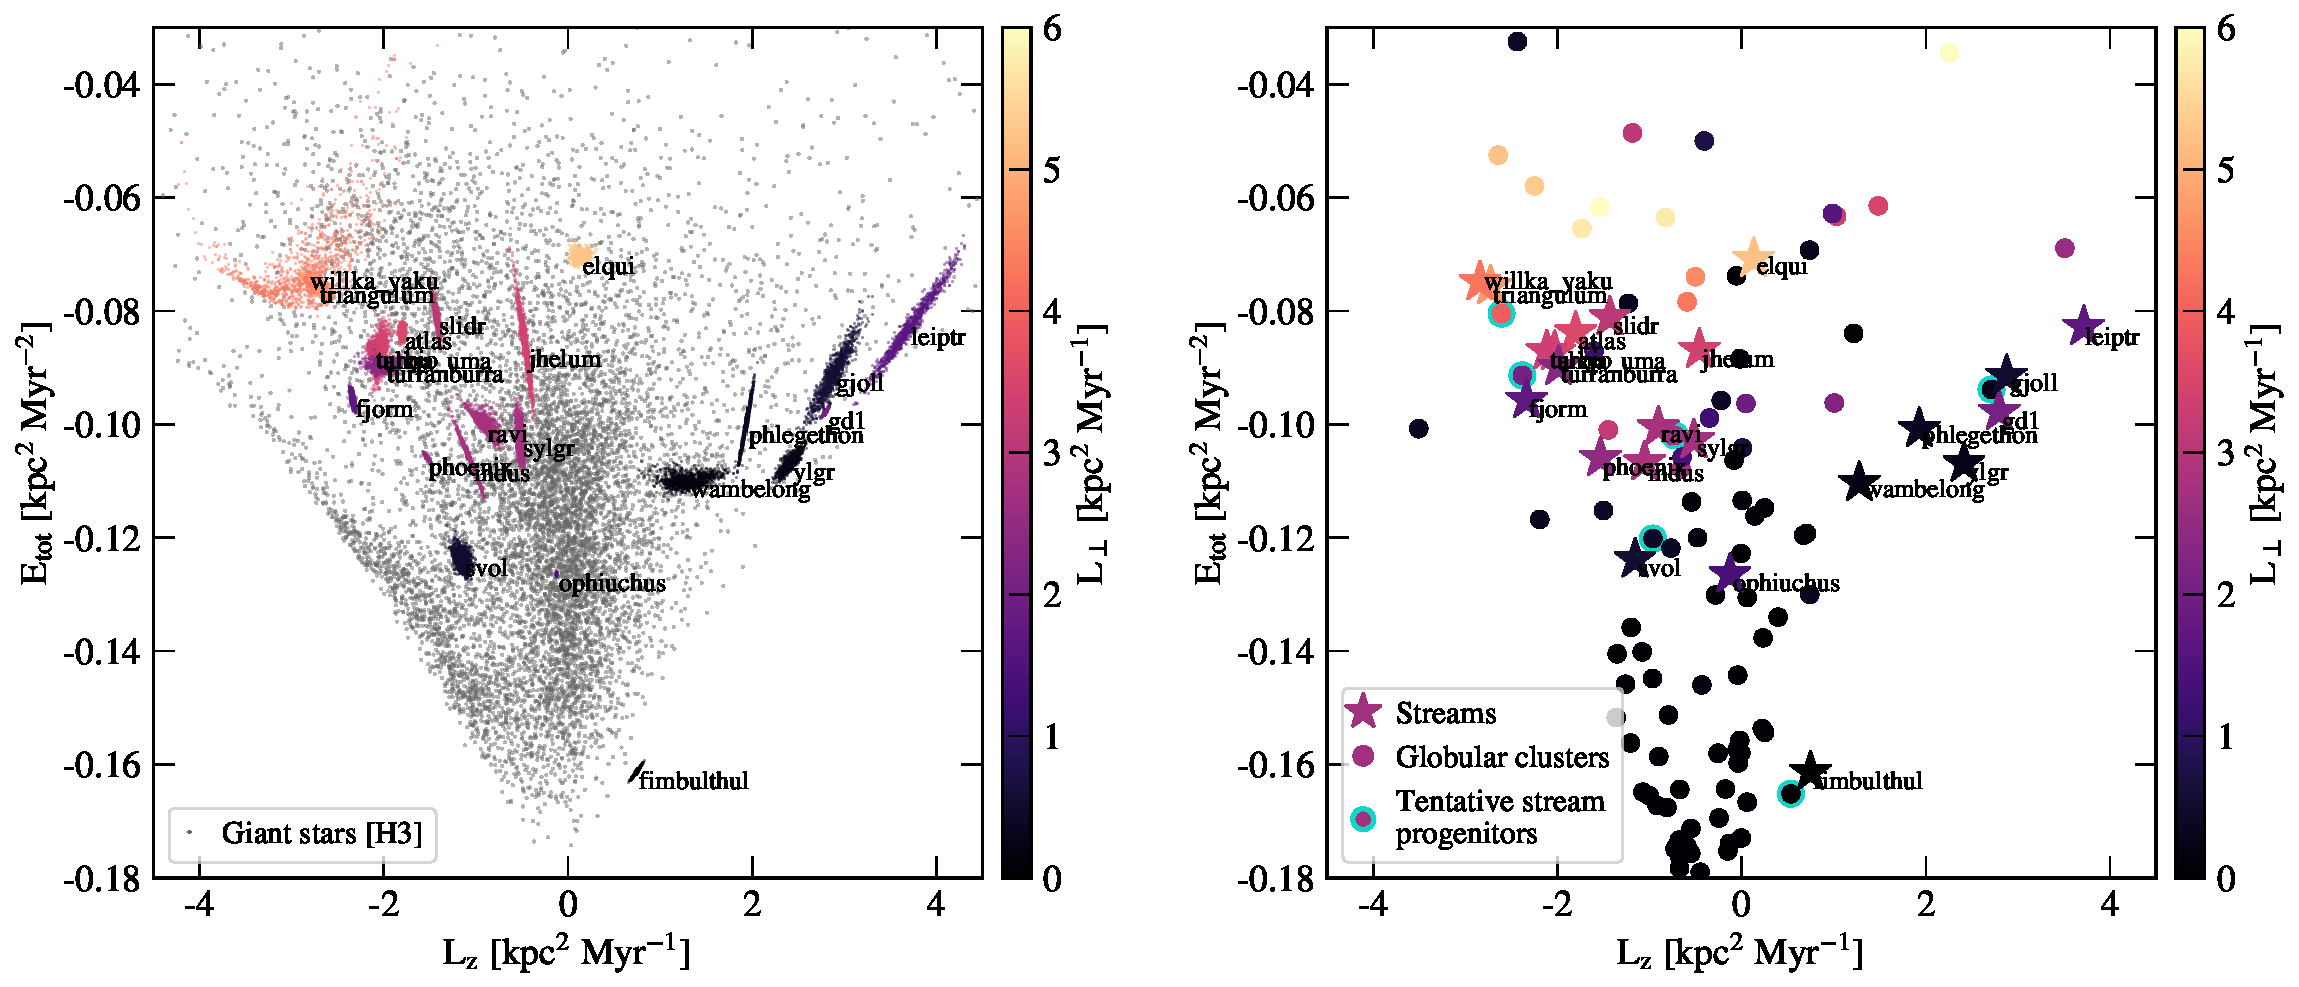
\includegraphics[width=\textwidth]{elz_streams.pdf}
\end{center}
\caption{The orbital phase space for cold stellar streams in the Milky Way (energy and angular momentum perpendicular to the disk, color-coded by the average orthogonal component of angular momentum), compared to field stars (left) and globular clusters (right).
Unlike stars and clusters, streams predominantly occupy tangential orbits and are more strongly clustered in phase space.
Globular clusters in close neighborhood of streams are plausible progenitors (cyan outlines).
}
\label{fig:elz}
\end{figure*}

\section{Streams in the phase space}
\label{sec:elz}
We present the phase-space distribution of Galactic streams in Figure~\ref{fig:elz}.
In the left panel, each stream is represented in energy and $L_z$ angular momentum with 1000 samples from the posterior distributions, while the medians of these distributions are shown as stars in the left panel.
In both panels, stream markers are color-coded by the in-plane component of the angular momentum, $L_\perp=\sqrt{L_x^2+L_y^2}$.
As a comparison, we include the phase-space distribution of giant stars from the H3 spectroscopic survey \citep[small black points on the left,][]{conroy2019}, and Galactic globular clusters \citep[small circles, colored by $L_\perp$,][]{baumgardt2019}.

The two most striking features of streams in the phase space are: (1) the amount of clustering, and (2) the lack of streams on radial orbits.
In contrast, the major feature in stars and globular clusters is the large population of objects on radial orbits with $L_z\approx0$, identified as debris from the Gaia Enceladus merger \citep{belokurov2018, helmi2018, naidu2020}.
Only two stellar streams are found on radial orbits, Ophiuchus and Elqui, and because of the large difference in their orbital energies they are likely unrelated.
Unlike stars and globular clusters, the rest of the streams are highly clustered in two groups, a retrograde containing 7 streams, and a prograde with 14 streams.

Most of the retrograde streams are found on a narrow locus from $(E_{\rm tot}, L_z)\approx(-0.08\,\ue,\allowbreak 4\,\ul)$ to $(E_{\rm tot}, L_z)\approx(-0.11\,\ue,\allowbreak 1\,\ul)$, which includes Leiptr, Gj\" oll, GD-1, Phlegethon, Ylgr, and Wambelong.
Fimbulthul is on the extension of this diagonal to lower energies.
With the exception of GD-1 and Leiptr, all retrograde streams have uniformly low $L_\perp\lesssim1\,\ul$.
This clustering indicates that the entire retrograde group shares a common origin.

The prograde group of streams shows additional structure with smaller clusters that include: (1) Triangulum and Willka Yaku at $L_z\approx-3\,\ul$, (2) Slidr, ATLAS, Aliqa Uma, Turbio, Turraburra, and Fjorm at $L_z\approx-2\,\ul$, and (3) Jhelum, Sylgr, Ravi, Indus, Phoenix, and Sv\" oll at $L_z\approx-1\,\ul$.
The in-plane angular momentum, decreases with $L_z$ and is approximately uniform within each small cluster.
The median energy of small clusters also decreases with $L_z$, however, so does the dispersion, such that the most radial clump spans a large range in energy levels.
Clustering on the prograde side also provides tantalizing evidence of common origin among stellar streams, which we explore further in \S\,\ref{sec:hosts}

Several streams also have orbits similar to that of a globular cluster, indicating a possible link.
These stream-cluster groups, outlined in cyan in the right panel of Figure~\ref{fig:elz}, appear close in energy and both components of the angular momentum.
We explore these connections further in \S\,\ref{sec:progenitors}.

% not really sure where to put this, but I think it is a cute point that I'd like to make and I think we will have room for it
At a given angular momentum, streams have preferentially lower energy orbits whereas field stars and globular clusters occupy a range of energy levels.
Interestingly, at the same amplitude of the angular momentum, $|L_z|$, prograde streams have higher energies than retrograde streams.
As spatial-overdensity searches are insensitive to the orbital direction, and proper-motion based searches are more sensitive to retrograde orbits, it is unlikely that the lack of retrograde streams at high energies is due to observational biases.
If confirmed as a reflection of the intrinsic orbital distribution by more complete stream samples, this asymmetry would suggest that objects on retrograde orbits are more resilient to tidal disruption, consistent with findings from numerical simulations \citep[e.g.,][]{find}.

\begin{figure}
\begin{center}
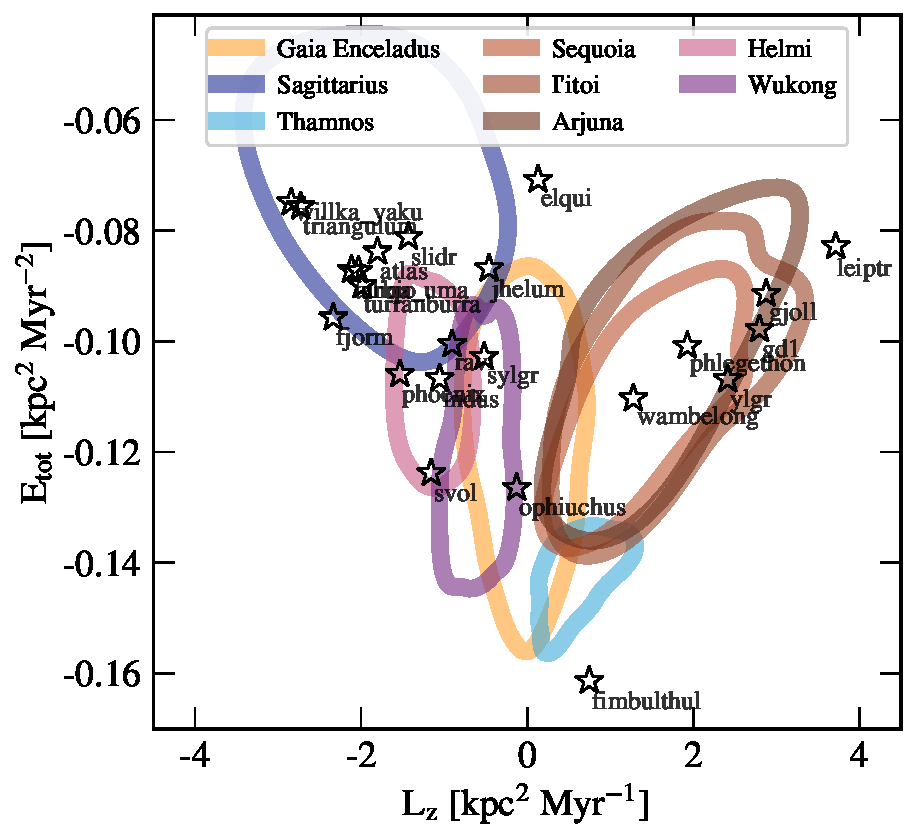
\includegraphics[width=\columnwidth]{stream_hosts.pdf}
\end{center}
\caption{
Stellar streams in our sample (stars) occupy areas of phase space where stars accreted from progenitor galaxies of the Milky Way have been identified (contours).
}
\label{fig:hosts}
\end{figure}

\subsection{Host galaxies}
\label{sec:hosts}
\citet{naidu2020} performed a detailed chemo-dynamical decomposition of stars observed with the H3 spectroscopic survey to identify structures in the Galactic halo of common origin.
In Figure~\ref{fig:hosts} we use contours of different colors to mark the phase-space distribution of ex-situ structures, most of which likely constitute distinct accretion events.
Specifically, we encompass the region where the average density for that component is higher than 20\,\% of its maximum in the space of energy and angular momentum.
The streams are overplotted as stars outlined in black.

Most of the streams have energies and angular momenta consistent with the distribution of one of the known halo substructures.
The high-energy group of retrograde streams is well aligned with debris from Sequoia, I'itoi, and Arjuna.
These three Milky Way progenitors differ in metallicity \citep{refs}, so it might be possible to further refine the streams' association with these structures based on their metallicity.
While GD-1 \citep[spectroscopic $\feh=-2.3$,][]{bonaca2020b}, Ylgr \citep[spectroscopic $\feh=-1.9$,][]{ibata2019}, and  Wambelong \citep[isochrone $\feh=-2.2$,][]{shipp2018} have low metallicities that can be plausibly associated with any of these progenitors, Gj\" oll \citep[spectroscopic $\feh=-1.5$,][]{hansen2020}, Leiptr \citep[isochrone $\feh=-1.6$,][]{ibata2019}, and Phlegethon \citep[spectroscopic $\feh=-1.6$,][]{ibata2018} are sufficiently metal-rich to favor association with Sequoia.

At low energies of the inner Galaxy, Fimbulthul lies beyond the region of energies and angular momenta surveyed by H3.
If accreted, Fimbulthul would have arrived to the Milky Way early to get settled so deep in the potential well.
Based on this timing argument, Fimbulthul may be associated with Thamnos, which was identified as a low-mass accretion event in the early Galaxy \citep{koppelman2019}.
This association can be confirmed with a more complete census of phase-space structures in the inner Galaxy.

On a high-energy radial orbit, Elqui appears unassociated with any of the Milky Way progenitors.
\citet{ji2020} found significant metallicity spread in Elqui, a telltale signature of a dwarf galaxy origin with an extended star-formation history compared to a globular clusters.
Combined with its orbital properties, this means that Elqui is tidal debris of a recently accreted dwarf galaxy.

On a low-energy radial orbit, Ophiuchus is likely associated with Gaia Enceladus.
Immediately upon its discovery, Ophiuchus was noted for its short extent and a low-density envelope \citep{bernard2015, sesar2015}.
Sources of perturbation present in the Milky Way, ranging from the Galactic bar \citep{price-whelan2016} to the Sagittarius dwarf galaxy \citep{lane2020}, have been proposed to explain the morphology of Ophiuchus.
More recently, \citet{carlberg2019} showed that streams originating from a host galaxy outside the Milky Way can develop similar low-density features.
Numerical simulations that take into account Ophiuchus' likely evolution within a host galaxy undergoing a radial merger might resolve the origin of its mysterious morphology.

- jhelum and indus: also spread in feh -> dwarf origin
- but similar orbits, and similar metallicity: likely different wraps
- similar angular momentum in all components, but difference in energy: due to orbital decay / dynamical friction?
-- are these individual pericentric stripping events?
- do we associate them w or as wukong or helmi? kind of right on the boundary

- svol, phoenix, ravi, sylgr -- helmi?

- willka yaku, triangulum, turbio -- cetus
- also ask rohan for cetus selection

- slidr, turranburra, fjorm, atlas, aliqa uma -- sgr locus, but at lower energy than most of the debris
- more loosely bound clusters, at lower energy orbits, why got disrupted?
- also note atlas aliqa uma linked by ting, spatially identified as separate bc a bit offset on the sky, but really one structure, just perturbed
- if came from sgr, probably due to that perturbation

Our results imply that the original host galaxy for a large fraction of stellar streams in the Galactic halo was not the Milky Way, but one of its lower-mass progenitors.
Tentative associations of streams and their host galaxies are listed in Table~\ref{table}.


\begin{figure*}
\begin{center}
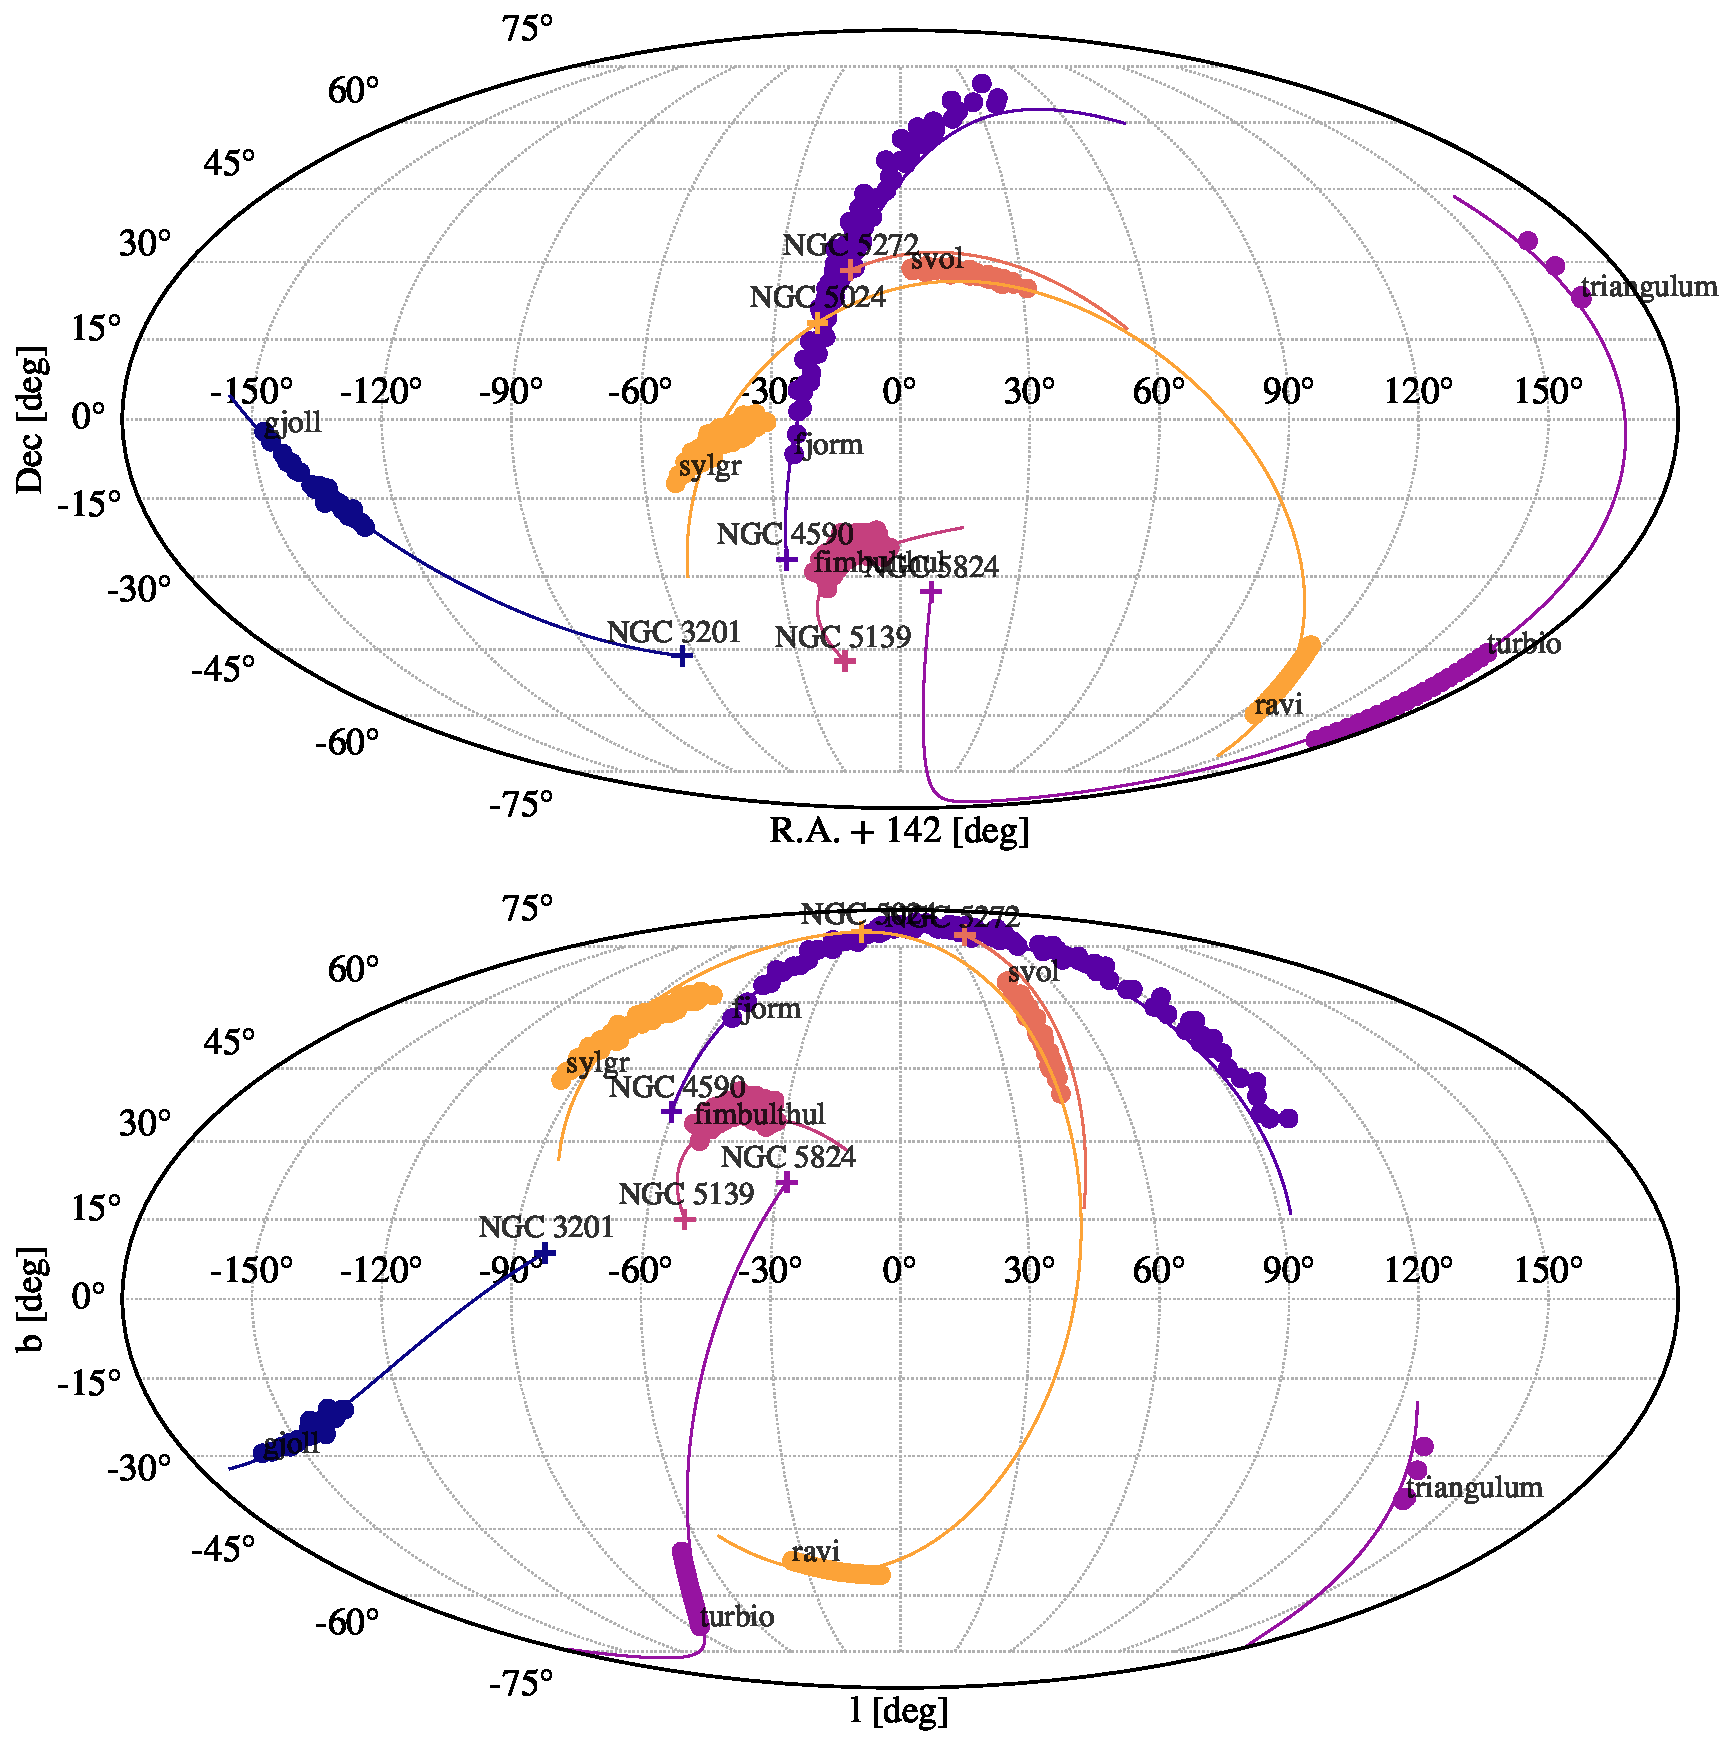
\includegraphics[width=\textwidth]{sky_orbits.pdf}
\end{center}
\caption{
Sky positions of stellar streams (circles) and globular clusters (crosses) that have similar orbital energies and angular momenta (see Figure~\ref{fig:elz}), shown in the equatorial coordinates in the top and galactic at the bottom.
Despite being spatially separated, these clusters are likely stream progenitors because their orbits (lines) connect them to the streams.
}
\label{fig:sky}
\end{figure*}

\subsection{Individual progenitors}
\label{sec:progenitors}
- fig 3
- omega cen fimbulthul from ibata (weaker gaia detection for the gap, not initially discovered bc close to the plane -- check if other chunks missing bc of not searching at low b)
- gjoll 3201 from hansen


\section{Discussion}
\label{sec:discussion}
- summary
- put table

implications for galaxy formation:
- meshes well w the accretion picture from stars, gc
- speculate on the lower energy than stars, gcs -- those got disrupted first?

special bc accreted:
- should have similar elz, clustering == metric of the grav potential
- difference in velocity dispersion depends whether cusp / core for dwarf streams, aggregate different in gc streams

puzzles / new handles on things?:
- why are streams discontinued?
- where are the opposite end counterparts for most of them?
- speculate on mass-loss episodes, scattering

future outlook

\vspace{0.5cm}
It is a pleasure to thank 

\software{
\package{Astropy} \citep{astropy, astropy:2018},
\package{gala} \citep{gala},
\package{IPython} \citep{ipython},
\package{matplotlib} \citep{mpl},
\package{numpy} \citep{numpy},
\package{scipy} \citep{scipy}
}

\bibliographystyle{aasjournal}
\bibliography{elz}


\end{document}